\chapter{Užívateľská dokumentácia}
\label{udok:chap}

V tejto kapitole si ukážeme možnosti používania našej aplikácie, tak ako aj popis jej samotného užívateľského rozhrania. Predtým si ale ešte musíme nainštalovať niektoré aplikácie potrebné k jej plnému využitiu.

\section{Inštalácia}
Našu aplikáciu nie je potrebné nijakým spôsobom inštalovať. Stačí otvoriť súbor \textit{USB\_Packet\_Analyzer.exe} v priečinku \textit{Release}, ktorý je súčasťou prílohy tejto práce. Podporovaná platforma našej aplikácie je momentálne iba Windows 10 64-bit verzie 20H2. Pre vytváranie súborov na analýzu si ale budeme musieť nainštalovať aplikácie USBPcap a Wireshark. V prípade, že nemáme záujem o analýzu paketov v reálnom čase, bude nám stačiť aplikácia USBPcap.

\subsection{USBPCap}
Aplikáciu USBPcap nainštalujeme podľa nasledujúcich krokov:
\begin{enumerate}
\item Prejdeme na stránku \uv{https://desowin.org/usbpcap/}.
\item V \textit{Download} časti klikneme na \uv{USBPcapSetup-1.5.4.0.exe}\footnote{Číslo sa môže líšť na základe aktuálnej verzie USBPCapu.}, čím začne sťahovanie USBPCap setupu.
\item Spustíme USBPCapSetup, ktorý sme stiahli v predchádzajúcom kroku, čo nám otvorí dialógové okno inštalácie.
\item Akceptujeme licenčné podmienky a klikneme na tlačidlo \uv{Next}. Opakujeme aj na ďalšej strane okna.
\item Necháme zaškrtnuté všetky komponenty a klikneme na \uv{Next}.
\item Zvolíme si priečinok do ktorého chceme USBPCap nainštalovať a klikneme na \uv{Install}.
\item Po inštalácii klikneme na \uv{Close}, čím inštalácia končí. Následne musíme ešte reštartovať počítač.
\end{enumerate}

\subsection{Wireshark}
Pre nainštalovanie Wiresharku budeme postupovať podľa nasledujúcich krokov:
\begin{enumerate}
\item Prejdeme na stránku \uv{https://www.wireshark.org/\#download}.
\item V časti \textit{Stabe Release (3.4.5)\footnote{Číslo sa môže líšť na základe aktuálnej verzie Wiresharku.}} klikneme na položku \uv{Windows Installer (64-bit)} a stiahneme inštalačný súbor Wiresharku.
\item Spustíme súbor, ktorý sme si stiahli v minulom kroku, čím sa nám otvorí dialógové okno inštalácie.
\item Klikneme na tlačidlo \uv{Next} a následne na tlačidlo \uv{Noted}.
\item Necháme zaškrtnuté všetky možnosti a klikneme na tlačidlo \uv{Next}.
\item V časti \uv{Create Shortcuts} zaškrtneme možnosti podľa osobných preferencií a klikneme na tlačidlo \uv{Next}.
\item Zvolíme si priečinok do ktorého chceme Wireshark nainštalovať a klikneme na tlačidlo \uv{Next}.
\item V prípade, že nemáme nainštalovaý Npcap, zaškrtneme možnosť na jeho nainštalovania a klikneme na tlačidlo \uv{Next}.
\item USBPCap by sme už mali mať nainštalovaný podľa predchádzajúceho návodu, takže len klikneme na tlačidlo \uv{Install}.
\item Po dokončení inštalácie klikneme na tlačidlo \uv{Next} a následne na tlačidlo \uv{Finish}.
\end{enumerate}

Aby sme vedeli spustiť zachytávanie paketov pomocou USBPcapu cez interface Wiresharku, prejdeme do priečinku v ktorom sme nainštalovali USBPcap a skopírujeme odtiaľ súbor \uv{USBPcapCMD.exe} do priečinku \uv{extcap} v adresári kde máme nainštalovaný Wireshark.



\section{Orientácia v GUI aplikácie}
Teraz si predstavíme užívateľské rozhranie aplikácie (obrázok~\ref{obr:kap6:gui}) a funkcionalitu jednotlivých tlačidiel. 

\begin{figure}[!htb]
	\centering
	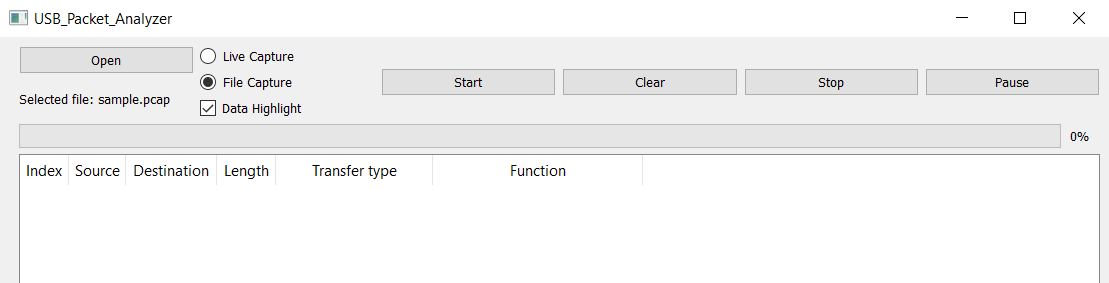
\includegraphics[width=\textwidth]{img/kap06_gui}
	\caption{Ukážka užívateľského rozhrania aplikácie.}
	\label{obr:kap6:gui}
\end{figure}

Teraz si postupne predstavíme jednotlivé tlačidlá:

\paragraph{Open} 
\hfill\break
Ako už samotný názov tlačidla napovedá, slúži na otváranie jednotlivých súborov, ktorých obsah budeme chcieť analyzovať.
Po jeho stlačení sa nám otvorí dialógové okno pomocou ktorého si zvolíme konkrétny pcap súbor. Akonáhle budeme mať daný súbor zvolený, pod tlačidlom bude vypísaný jeho názov.

\paragraph{Live Capture/File Capture}
\hfill\break
Nasleduje výber medzi Live Capture/File Capture pomocou RadioButtonov. File Capture reprezentuje analýzu ukončeného súboru, zatiaľ čo Live Capture podporuje analýzu súboru \uv{v reálnom čase}, takže je do súboru počas analýzy pripísať nové údaje, ktoré budú následne spracované aplikáciou.

\paragraph{Data Highlight}
Je CheckBox pomocou ktorého si užívateľ zvolí, či chce mať farebne zvýraznené položky v hexdumpe na základe ich významu alebo chce mať čistý hexdump bez farebného označenia. 

\paragraph{Start}
\hfill\break
Týmto tlačidlom spustíme analýzu zvoleného súboru. Ak sa navyše jedná o File Capture, progress bar pod tlačidlami nám percentuálne ukazuje akú časť súboru už máme spracovanú. Akonáhle progress bar dosiahne 100\%, celý súbor máme úspešne spracovaný a všetky základné informácie jednotlivých paketov (index, dĺžka, typ prenosu, atď.) sa zobrazia nižšie, pričom automaticky nás to posunie na úroveň posledného paketu. V prípade Live Capture to bude vyzerať podobne, ale progress bar nám momentálne nebude ukazovať percentuálnu časť spracovania súboru (pretože tá sa môže neustále meniť). Takisto nás to po odkončení analýzy posunie na úroveň aktuálneho paketu a to sa deje vždy keď sú do analýzy pridané nové pakety.

\paragraph{Clear}
\hfill\break
Toto tlačidlo nám vyčistí plochu do ktorej sú vyobrazované základné informácie jednotlivých paketov.

\paragraph{Stop}
\hfill\break
Toto tlačidlo je navrhnuté na používanie pri Live Capture kedy ukončí čítanie aktuálneho súboru a tým znemožní vyobrazenie nových paketov. Zároveň je tým znemožnená akákoľvek ďalšia analýza súborov. Toto tlačidlo užívateľ použije v prípade, že nemá záujem o analýzu nových paketov a stačia mu tie, ktoré má momentálne zobrazené v aplikácii.

\paragraph{Pause}
\hfill\break
Tlačidlo je tatiež navrhnuté na používanie pri Live Capture, kedy ním užívateľ dáva najavo, že chce pozastaviť pridávanie nových paketov na analýzu. Po jeho kliknutí sa nápis tlačidla zmení na \uv{Continue}, čím získava opačnú funkcionalitu -- obnovenie pridávania paketov. Všetky pakety, ktoré boli v súbore v intervale medzi stlačením Pause a Continue sú vynechané a pridávanie pokračuje od nasledujúcich paketov.



\section{Používanie aplikácie}
V tejto sekcii si ukážeme prácu s aplikáciou a ako vykonať File aj Live Capture analýzu. 

\subsection{Vytváranie pcap súborov}
Postup vytvárania súboru sa bude líšiť vzhľadom na to o aký druh analýzy máme záujem. Obecne je intuitívnejšie pracovať v oboch prípadoch s Wiresharkom ale v prípade, že si ho nechceme nainštalovať a máme záujem využívať iba možnosť File Capture, ukážeme si aj prácu s USBPcapom.

\subsubsection{File Capture}
Na vytvorenie pcap súboru pre File Capture máme na výber použiť USBPCap alebo Wireshark.

\paragraph{USBPcap}
Ak sa rozhodneme použiť USBPCap, postupujeme nasledovne:
\begin{enumerate}
\item Do tých USB portov, ktoré budeme chcieť počas zachytávania paketov sledovať pripojíme ľubovoľné HID zariadenie.
\item Zapneme USBPcap command line aplikáciu cez \textit{USBPcapCMD.exe}.
\item\label{kap6:sec:usbpcap_vyber_portov} Pomocou čísel si zvolíme USB porty, v ktorých máme zapojené zariadenia. Príklad vidíme na obrázku~\ref{obr:kap6:usbpcap_ports}, kde sú to porty 1 a 3.

\begin{figure}[!htb]
	\centering
	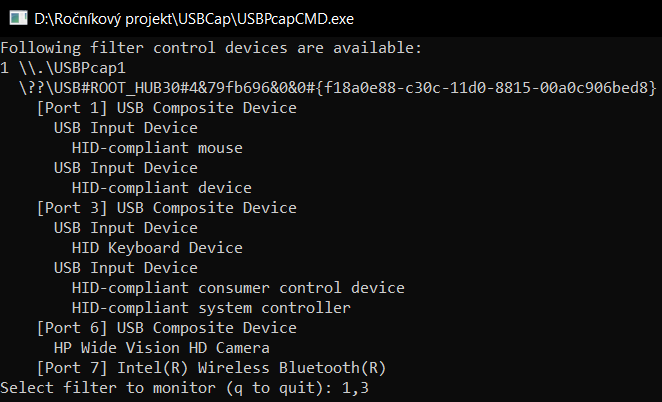
\includegraphics[width=12cm]{img/kap06_usbpcap_ports}
	\caption{Príklad vybratia portov 1 a 3 v aplikácii USBPcap.}
	\label{obr:kap6:usbpcap_ports}
\end{figure}

\item Následne si zvolíme meno súboru do ktrého chceme pakety zachytiť a stlačíme Enter. Vybehne nám \textit{Kontrola používateľských kont} v ktorej musíme povoliť USBPcap aplikácii vykonávanie zmien v zariadení. Predtým než to ale potvrdíme, odpojíme zariadenia zo všetkých USB portov, ktoré sme si zvolili vyššie. Toto robíme z dôvodu toho, aby sme už pri zachytávaní komunikácie dostali od zariadenia paket obsahujúci jeho HID Report Descriptor. V prípade, že zariadenia neodpojíme budeme mať síce zachytené všetky ostatné descriptory poslané počas konfigurácie, ale nebudeme schopní vykonať sémantickú analýzu inputu zariadení.
\item Po povolení vykonávaní zmien pripojíme do daných portov zariadenia, s ktorými chceme sledovať komunikáciu a môžeme s nimi vykonávať akcie, ktoré chceme mať zachytené.
\item Akonáhle chceme s analýzou skončiť, stlačíme klávesu \uv{q} a tým zároveň uončíme USBPCap. Momentálne by sme mali nájť náš súbor v priečinku v ktorom sa nachádza \textit{USBPcapCMD.exe}.
\end{enumerate}

USBPCap má ešte jednu nevýhodu -- zachytí konfiguráciu zariadení na všetkých USB portoch (aj tých, ktoré sme si v kroku~\ref{kap6:sec:usbpcap_vyber_portov} nezvolili). Samotnú komunikáciu s nimi už ale nesleduje.

\paragraph{Wireshark}
\label{kap6:sec:wireshark:file_capture}
V prípade použitia Wiresharku na vytváranie pcap sborov budeme nasledovať podľa týchto krokov:
\begin{enumerate}
\item Zapneme Wireshark aplikáciu cez \textit{Wireshark.exe}.
\item Upravíme nastavenia USBPCapu stlačením na sivé koliesko vedľa jeho názvu v oblasti \textit{Capture} dole (obrázok~\ref{obr:kap6:wireshark_usbpcap_settings}).

\begin{figure}[!htb]
	\centering
	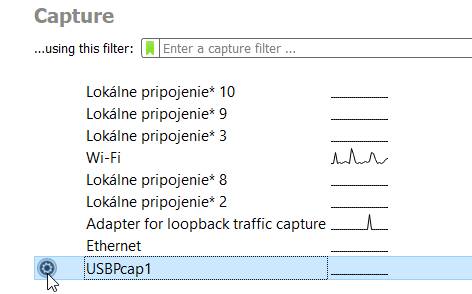
\includegraphics[width=10cm]{img/kap06_wireshark_usbpcap_settings}
	\caption{Ikona nastavenia USBPcapu vo Wiresharku.}
	\label{obr:kap6:wireshark_usbpcap_settings}
\end{figure}

\item Stlačíme tlačidlo \textit{Restore Defaults} a zašktrneme možnosť \textit{Capture from newly connected devices}. Bohužiaľ, pre uloženie týchto nastavení musíme spustiť jedno zachytávanie takže klikneme na tlačidlo \textit{Start} a potvrdíme \textit{Kontrolu používateľských kont}. Teraz môžeme toto zachytávanie zrušiť cez červený štvorec v hornej lište Wiresharku. Nastavenia sa nám týmto uložili a pokiaľ ich nebudeme chcieť zmeniť, nebudeme musieť tento krok už opakovať.
\item Teraz si vo Wiresharku cez možnosť \textit{Capture}$\rightarrow$\textit{Options} zaškrtneme v položke \textit{Input} možnosť USBPcap (obrázok~\ref{obr:kap6:wireshark_options_input}) a v položke \textit{Output} zvolíme možnosť \textit{pcap} a cez tlačidlo \textit{Browse} si vyberieme kde chceme uložiť súbor do ktorého budeme zachytávať komunikáciu (obrázok~\ref{obr:kap6:wireshark_options_output}).

\begin{figure}[!htb]
\centering
\begin{subfigure}{\textwidth}
  \centering
  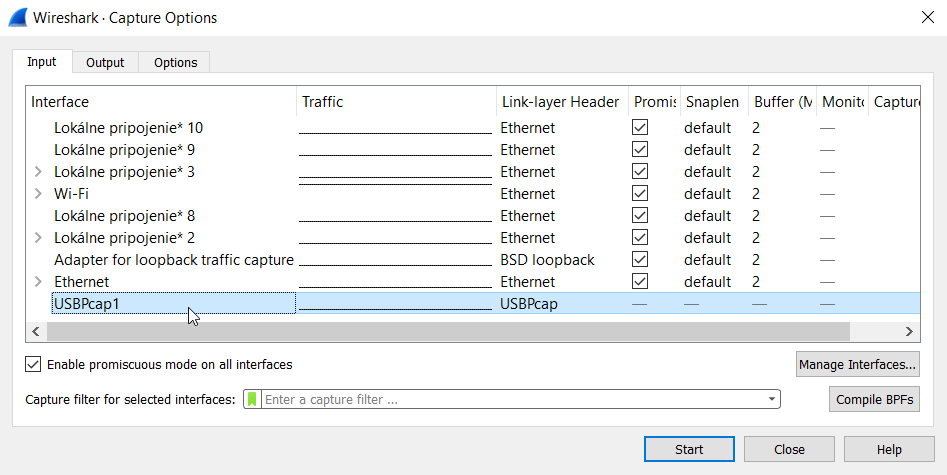
\includegraphics[width=\textwidth]{img/kap06_wireshark_options_input}
  \caption{Ukážka nastavenia inputu USBPcapu vo Wiresharku}
  \label{obr:kap6:wireshark_options_input}
\end{subfigure}
\begin{subfigure}{\textwidth}
  \centering
  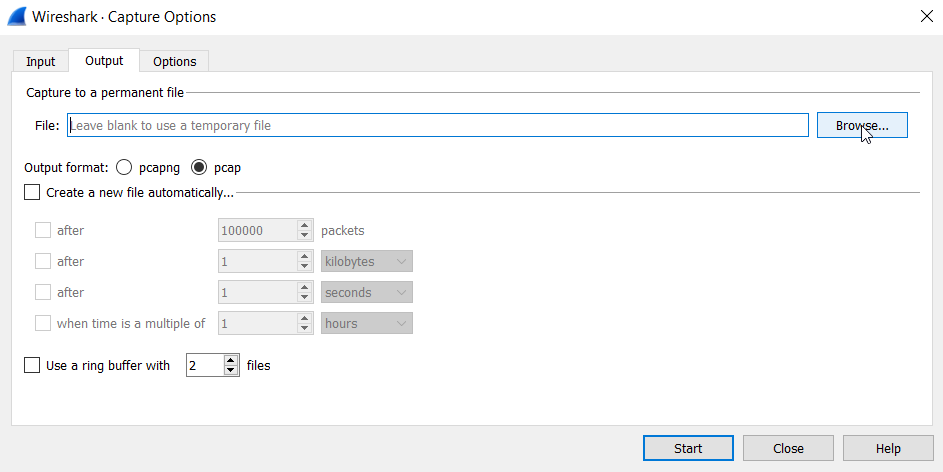
\includegraphics[width=\textwidth]{img/kap06_wireshark_options_output}
  \caption{Ukážka nastavenia outputu USBPcapu vo Wiresharku}
  \label{obr:kap6:wireshark_options_output}
\end{subfigure}
\caption{Ukážka nastavenia inputu a outputu USBPcapu vo Wiresharku}
\label{obr:kap6:wireshark_options_input_output}
\end{figure}

\item Skontrolujeme, že máme odpojené všetky zariadenia s ktorými chceme zachytávať komunikáciu a stlačíme tlačidlo \textit{Start}.
\item V momente keď budeme chcieť zachytávanie ukončiť, klikneme na červený štvorec v hornej lište Wiresharku.
\end{enumerate}

\subsubsection{Live Capture}
Na vykonanie Live Capture analýzy budeme potrebovať použiť aplikáciu Wireshark. Budeme postupovať pomocou rovnakých krokov ako pri File Capture~\ref{kap6:sec:wireshark:file_capture} s tou výnimkou, že teraz budeme mať počas zachytávania zapnutú aj našu aplikáciu ktorá bude vyobrazovať aktuálny stav súboru spolu s Wiresharkom.



\subsection{Príklad analýzy}
Momentálne si ukážeme konkrétny príklad File Capture analýzy na súbore \textit{sample.pcap}, ktorý je súčasťou prílohy k tejto práci. Budeme postupne zachytávať komunikáciu s 3 zariadeniami ukázanými na obrázku~\ref{obr:kap6:devices}:

\begin{figure}[!htb]
\centering
\begin{subfigure}{.4\textwidth}
  \centering
  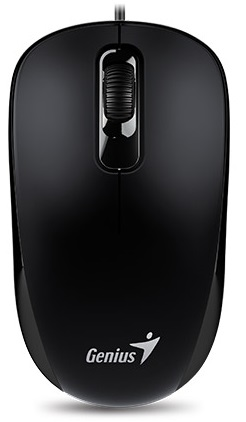
\includegraphics[width=.4\linewidth]{img/genius_mys.jpg}
  \caption{Fotka genius myši prevzatá z oficiálnej genius stránky~\cite{genius_mouse_pic}.}
  \label{obr:kap6:genius:mouse:pic}
\end{subfigure}%
\begin{subfigure}{.6\textwidth}
  \centering
  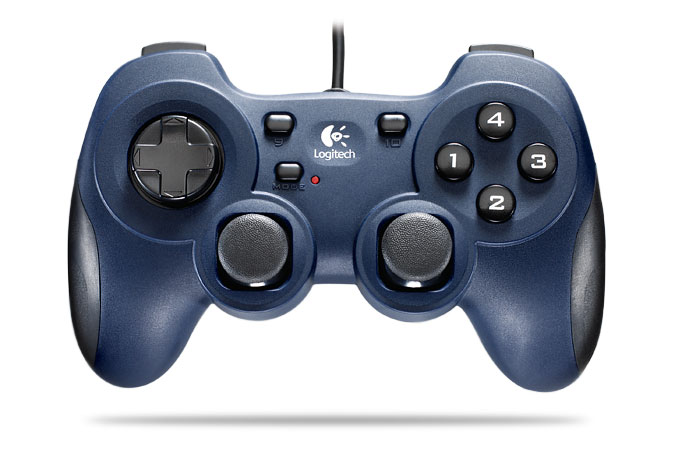
\includegraphics[width=.6\linewidth]{img/kap06_joystick}
  \caption{Fotka logitech joysticku prevzatá zo stránky obchodu~\cite{logitech_joystick_pic}.}
  \label{obr:kap6:joystick_obr}
\end{subfigure}
\begin{subfigure}{\textwidth}
  \centering
  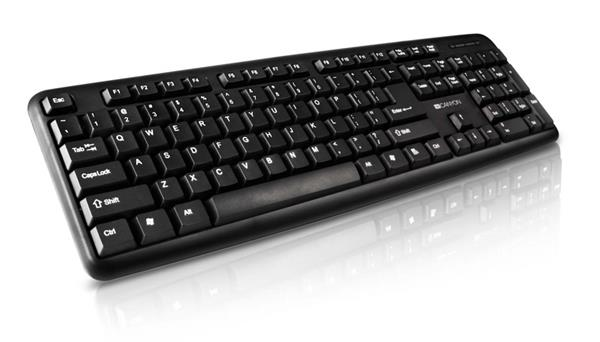
\includegraphics[width=\textwidth]{img/kap06_keyboard}
  \caption{Fotka CANYON klávesnice prevzatá zo stránky obchodu~\cite{canyon_keyboard_pic}.}
  \label{obr:kap6:keyboard_obr}
\end{subfigure}
\caption{Ukážka zariadení s ktorými budeme zachytávať komunikáciu.}
\label{obr:kap6:devices}
\end{figure}


Počas zachytávania sme vykonali nasledujúce:
\begin{enumerate}
\item Do USB portu sme pripojili zariadenie myši.
\item Stlačili sme ľavé tlačidlo myši.
\item Stlačili sme pravé tlačidlo myši.
\item Posunuli sme koliekom myši smerom dole.
\item Vykonali sme pohyb s myšou a naásledne ju odpojili.
\item Pripojili sme zariadenie klávesnice.
\item Stlačili a pustili sme tlačidlo \uv{A}.
\item Stlačili a podržali sme tlačidlo \uv{C} a potom tlačidlo \uv{D}, následne sme pustili tlačidlo \uv{C} a potom \uv{D}.
\item Stlačili a pustili sme tlačidlo \uv{Tab}.
\item Do druhého USB portu sme pripojili zariadenie joysticku.
\item Na joysticku sme stlačili s pustili sme tlačidlo \uv{1} a následne tlačidlo \uv{8}.
\item Stlačili a pustili sme niekoľko tlačidiel naraz.
\item Vykonali sme pohyb analógom.
\item Ukončili sme zachytávanie.
\end{enumerate}

Teraz si otvoríme našu aplikáciu, pomocou tlačilda \uv{Open} si vyberieme súbor s vyššie opísanou zachytenou komunikáciou a stlačíme tlačidlo \uv{Start}. Pre bližšiu analýzu jednotlivých paketov dvojklikneme na riadok, ktorý daný paket reprezentuje. To má za následok vytvorenie pop-up okna (obrázok~\ref{obr:kap6:uk_popup}), ktoré má nasledujúce rozloženie:
\begin{itemize}
\item Vľavo hore máme vyobrazenú stromovú štruktúru, ktorá detailnejšie opisuje hlavičku paketu.
\item Vpravo hore je vyobrazená stromová štruktúra reprezentujúca sémantický význam zyvškových dát paketu.
\item Vľavo dole máme stromovú štruktúru opisujúcu farby v Color Map pre jenoduchšiu orientáciu v hexdumpe.
\item Vedľa Color Map sa nachádza daný hexdump, pričom tabuľka vľavo vyobrazuje znaky v ich hexadecimálnej podobe a tabuľka vpravo vyobrazuje dané znaky v ich tlačiteľnej podobe.
\end{itemize}

\begin{figure}[!htb]
	\centering
	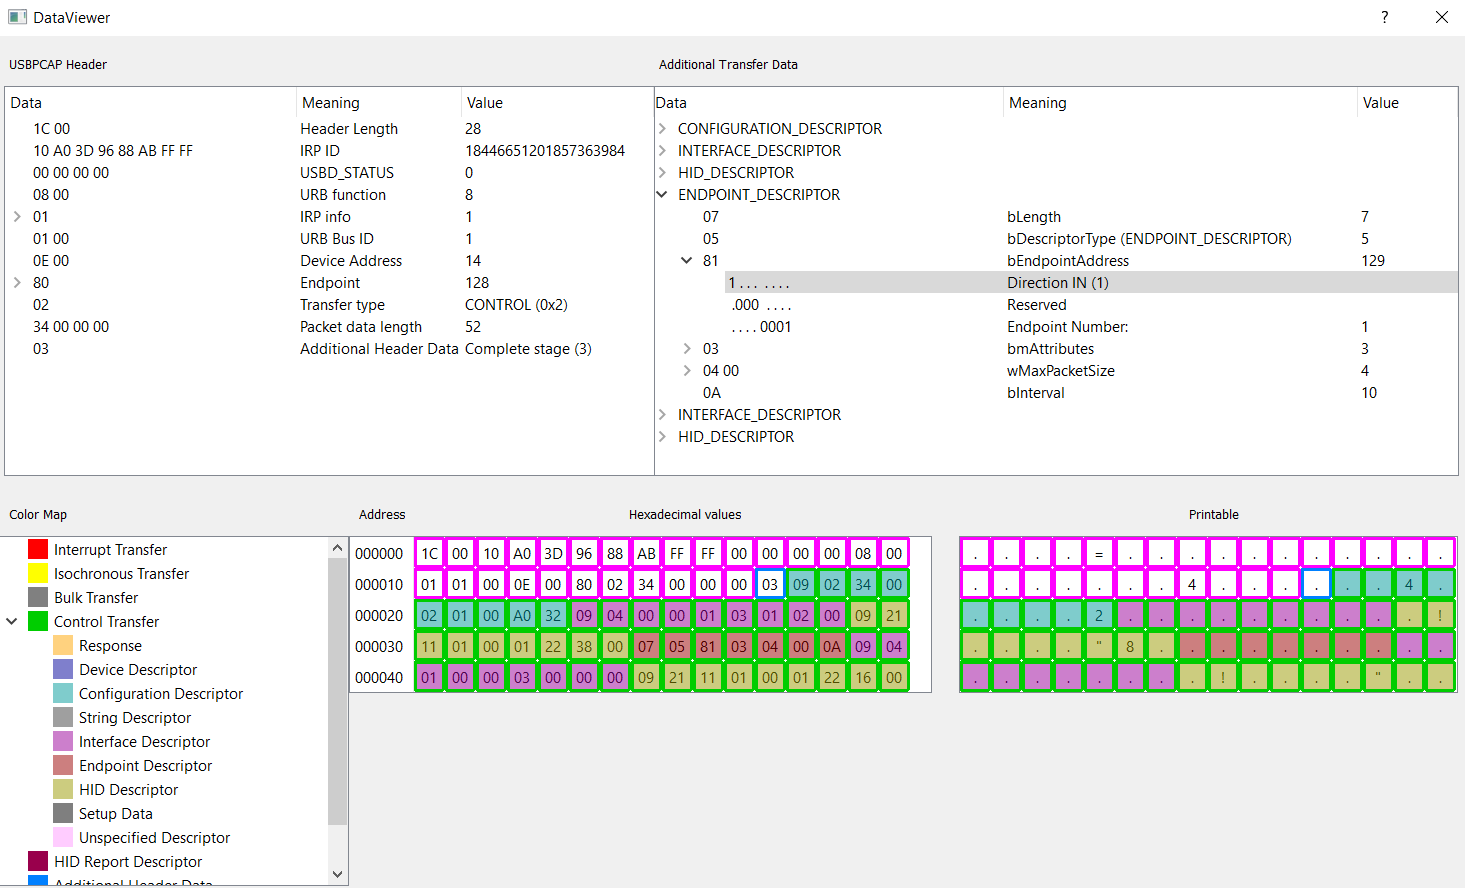
\includegraphics[width=\textwidth]{img/kap06_uk_popup}
	\caption{Ukážka pop-up okna aplikácie.}
	\label{obr:kap6:uk_popup}
\end{figure}

Momentálne si už len ukážeme zopár obrázkov analýzy vyššie spomínanej komunikácie.

\begin{figure}[!htb]
	\centering
	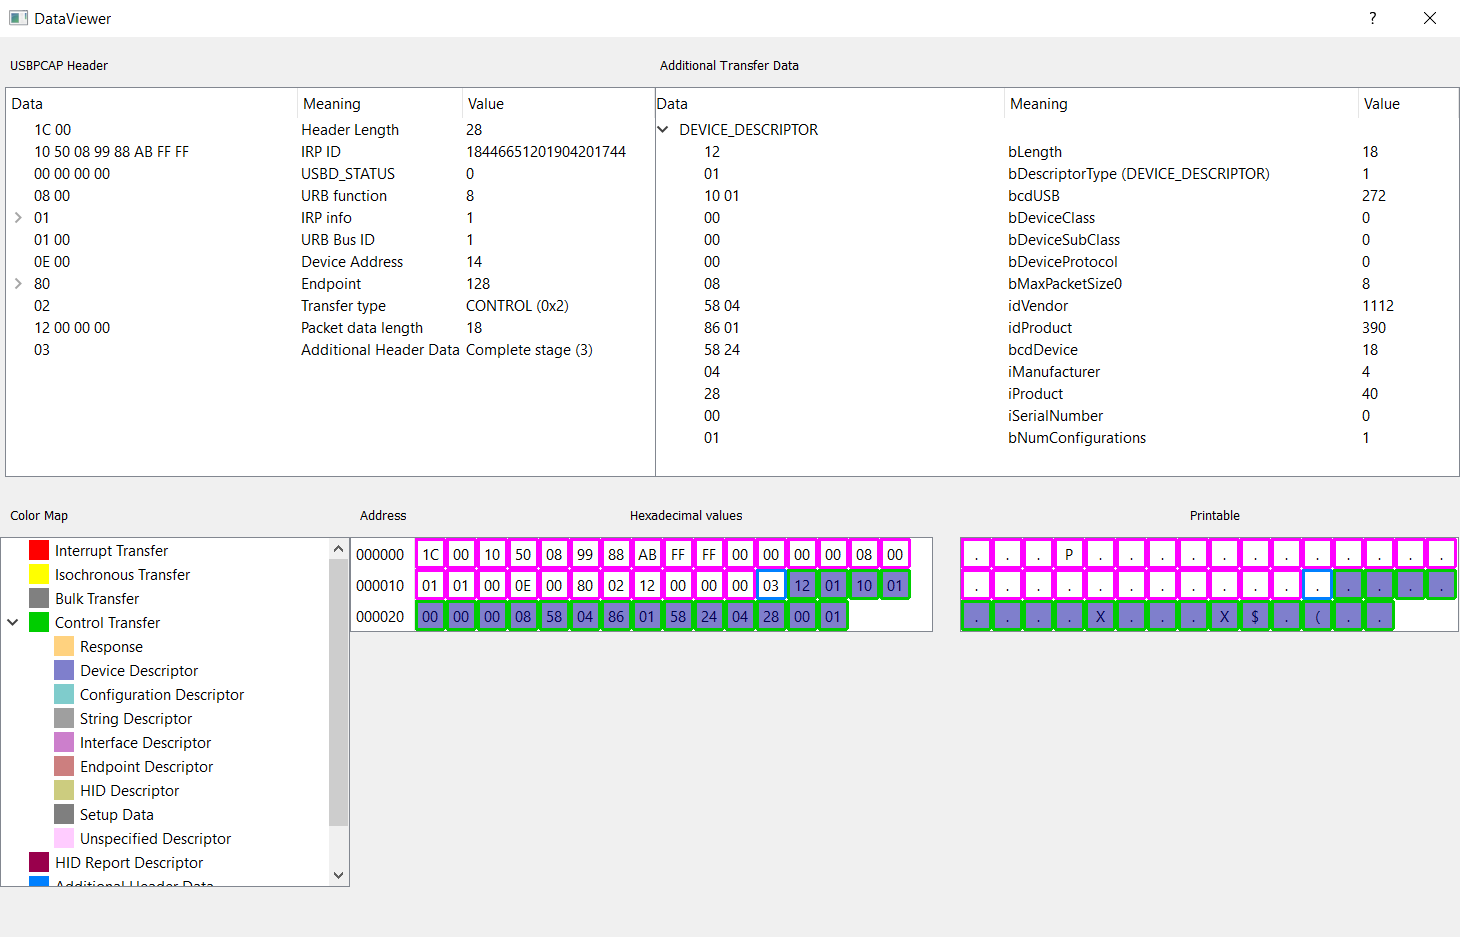
\includegraphics[width=\textwidth]{img/kap06_device_desc}
	\caption{Ukážka Device Descriptoru myši.}
	\label{obr:kap6:uk_device_desc}
\end{figure}

\begin{figure}[!htb]
	\centering
	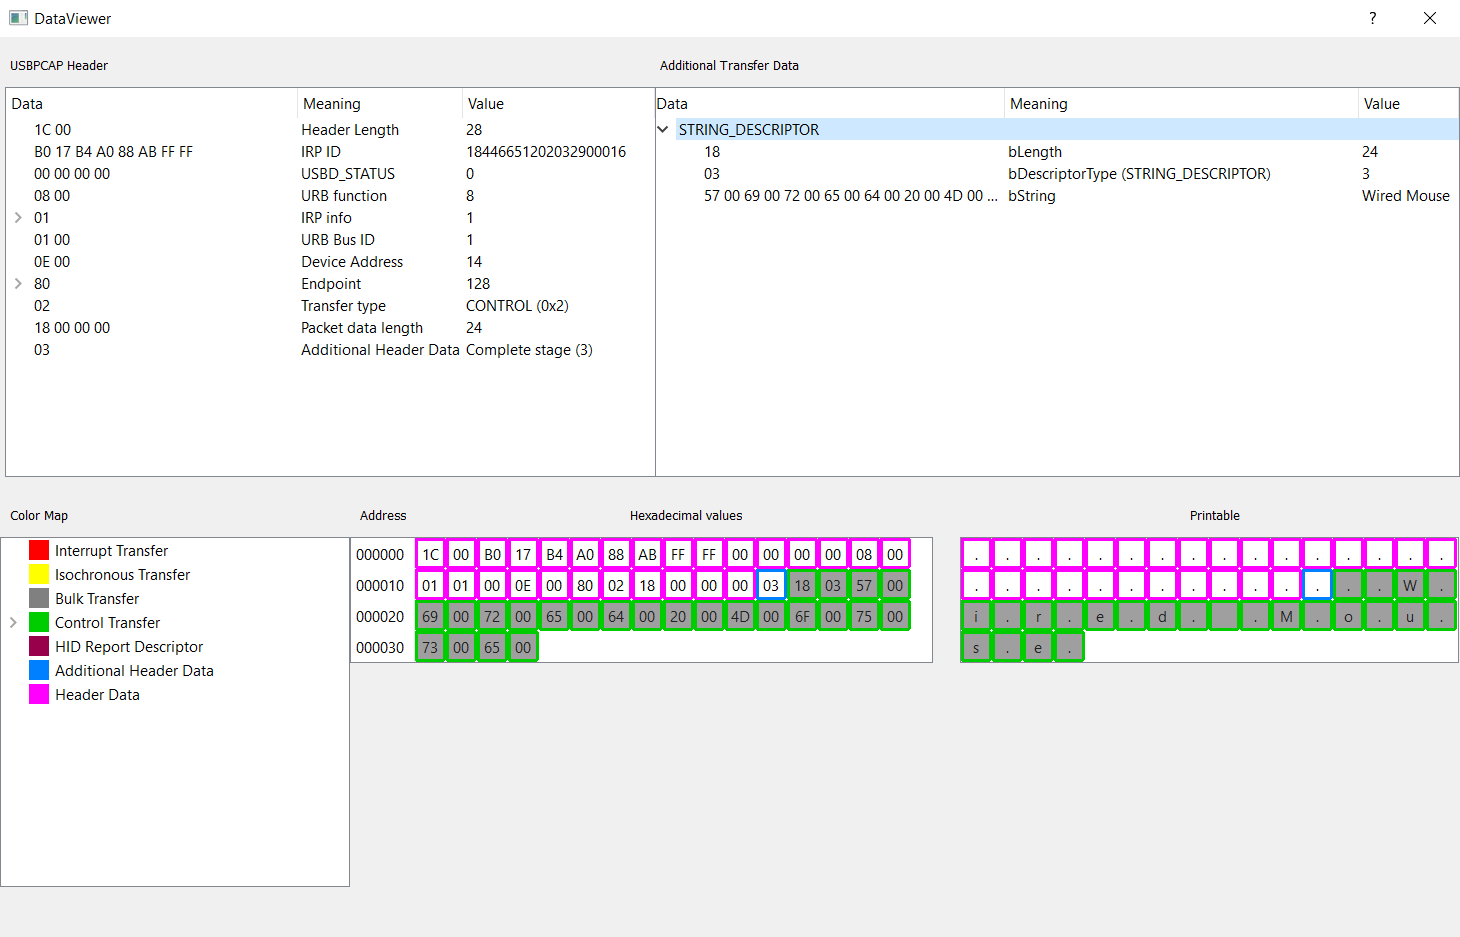
\includegraphics[width=\textwidth]{img/kap06_uk_string_descriptor}
	\caption{Ukážka String Descriptoru myši.}
	\label{obr:kap6:uk_string_desc}
\end{figure}

\begin{figure}[!htb]
	\centering
	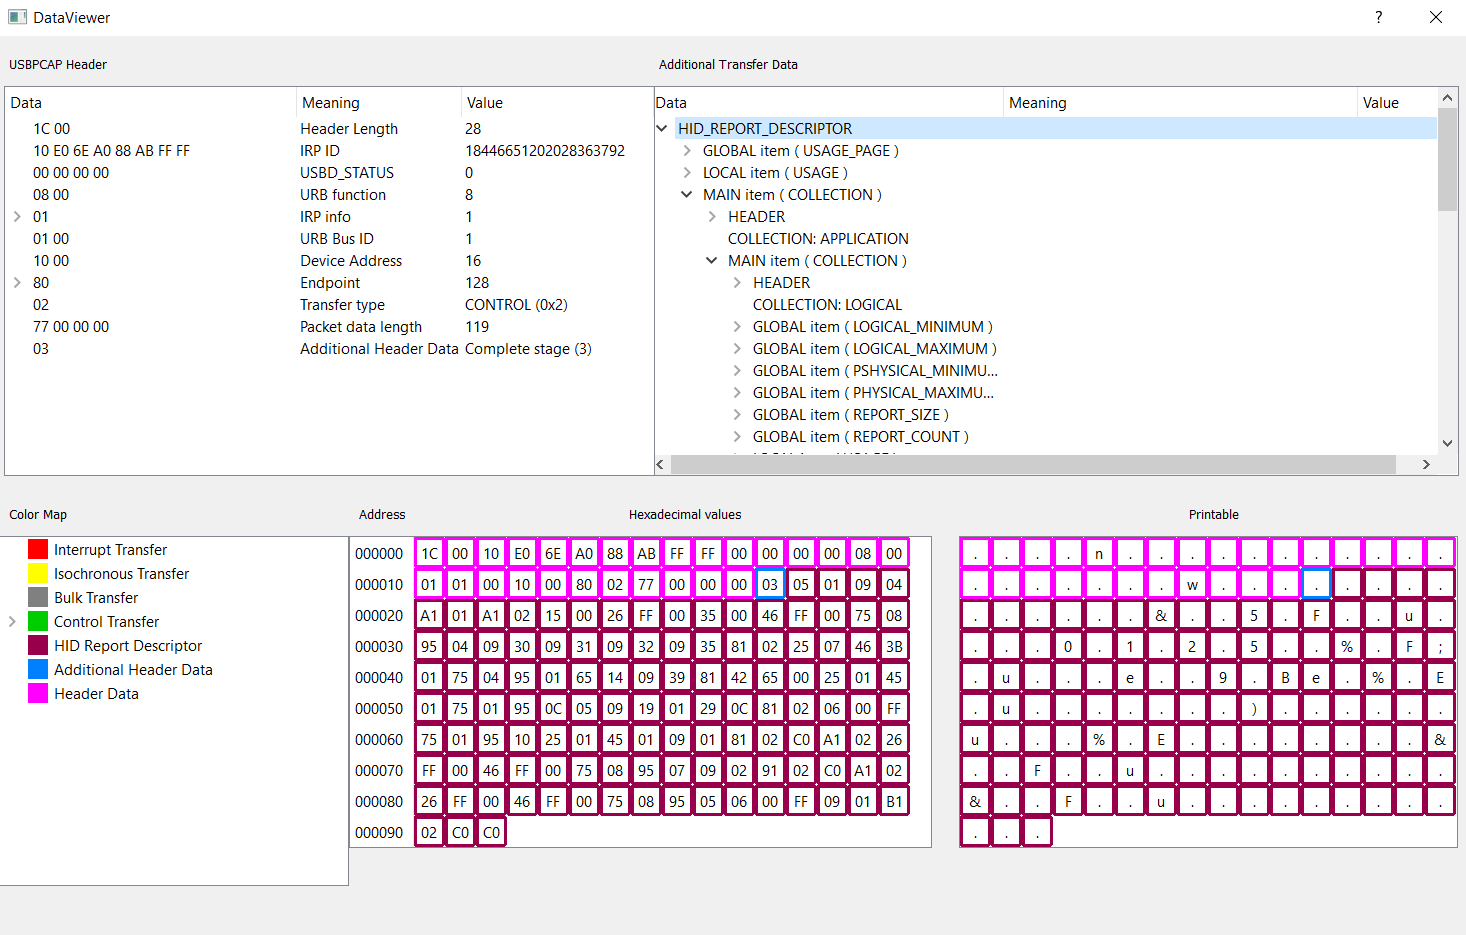
\includegraphics[width=\textwidth]{img/kap06_uk_report_desc}
	\caption{Ukážka Report Descriptoru joysticku.}
	\label{obr:kap6:uk_report_desc}
\end{figure}

\begin{figure}[!htb]
	\centering
	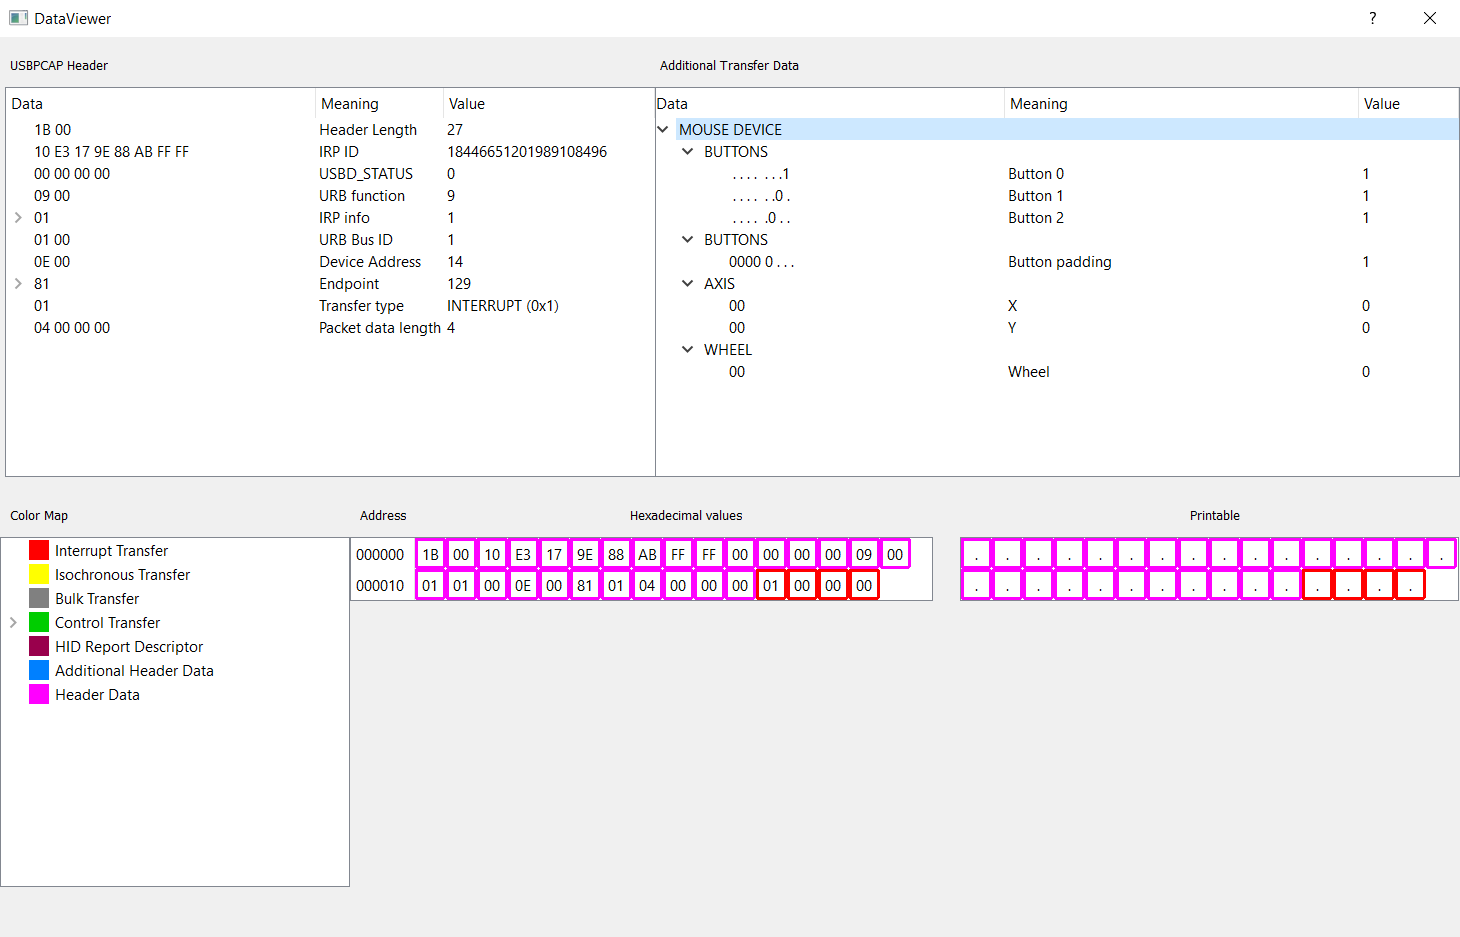
\includegraphics[width=\textwidth]{img/kap06_uk_mouse}
	\caption{Ukážka inputu myši.}
	\label{obr:kap6:uk_input_mouse}
\end{figure}

\begin{figure}[!htb]
	\centering
	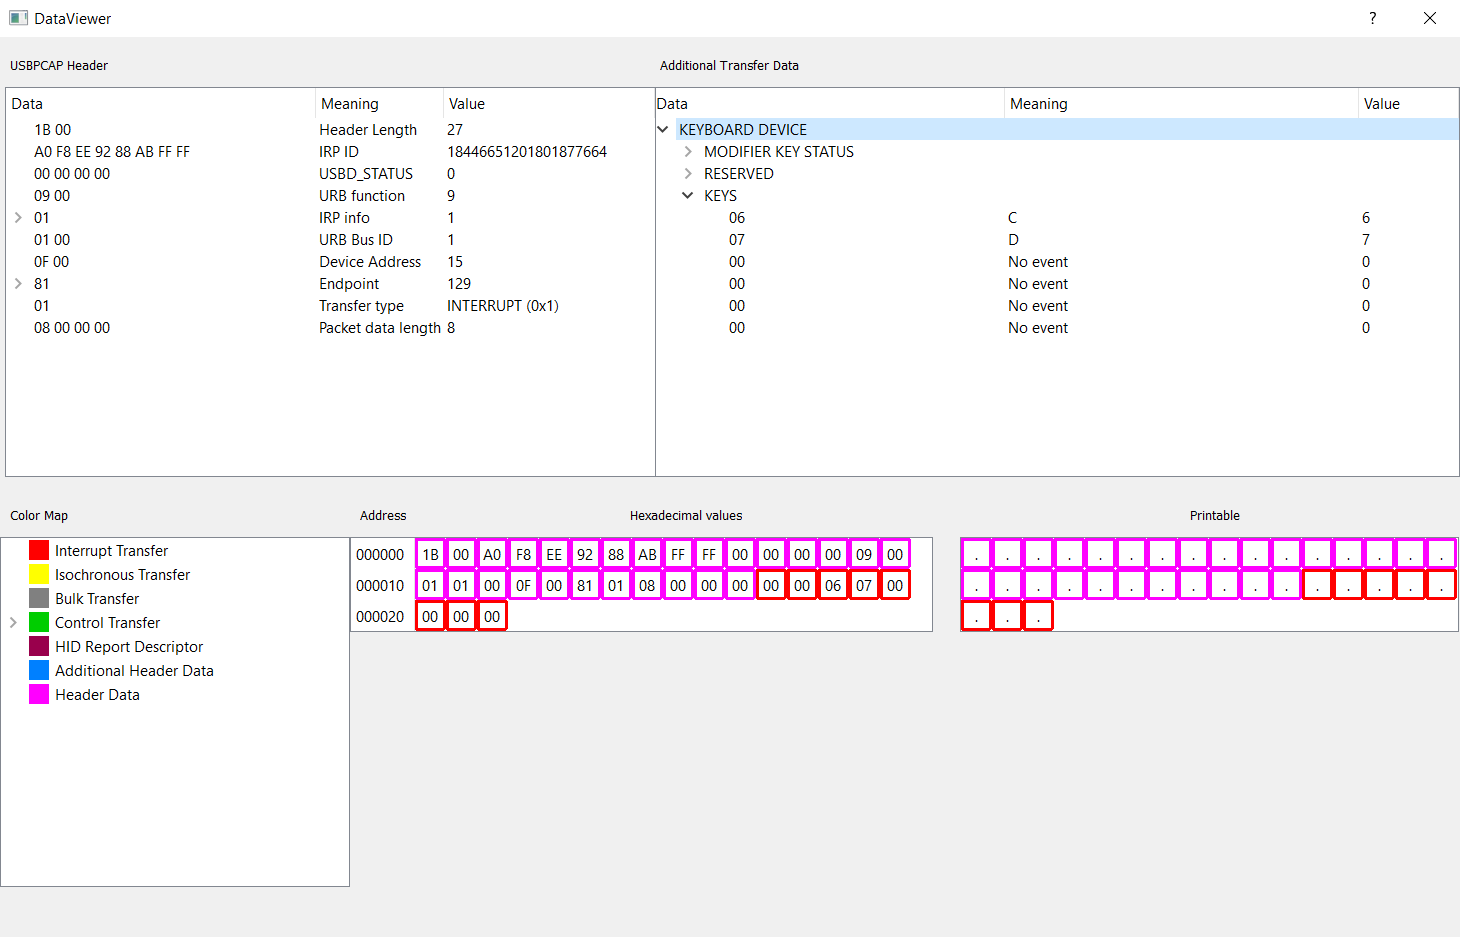
\includegraphics[width=\textwidth]{img/kap06_uk_keyboard}
	\caption{Ukážka inputu klávesnice.}
	\label{obr:kap6:uk_input_keyboard}
\end{figure}

\begin{figure}[!htb]
	\centering
	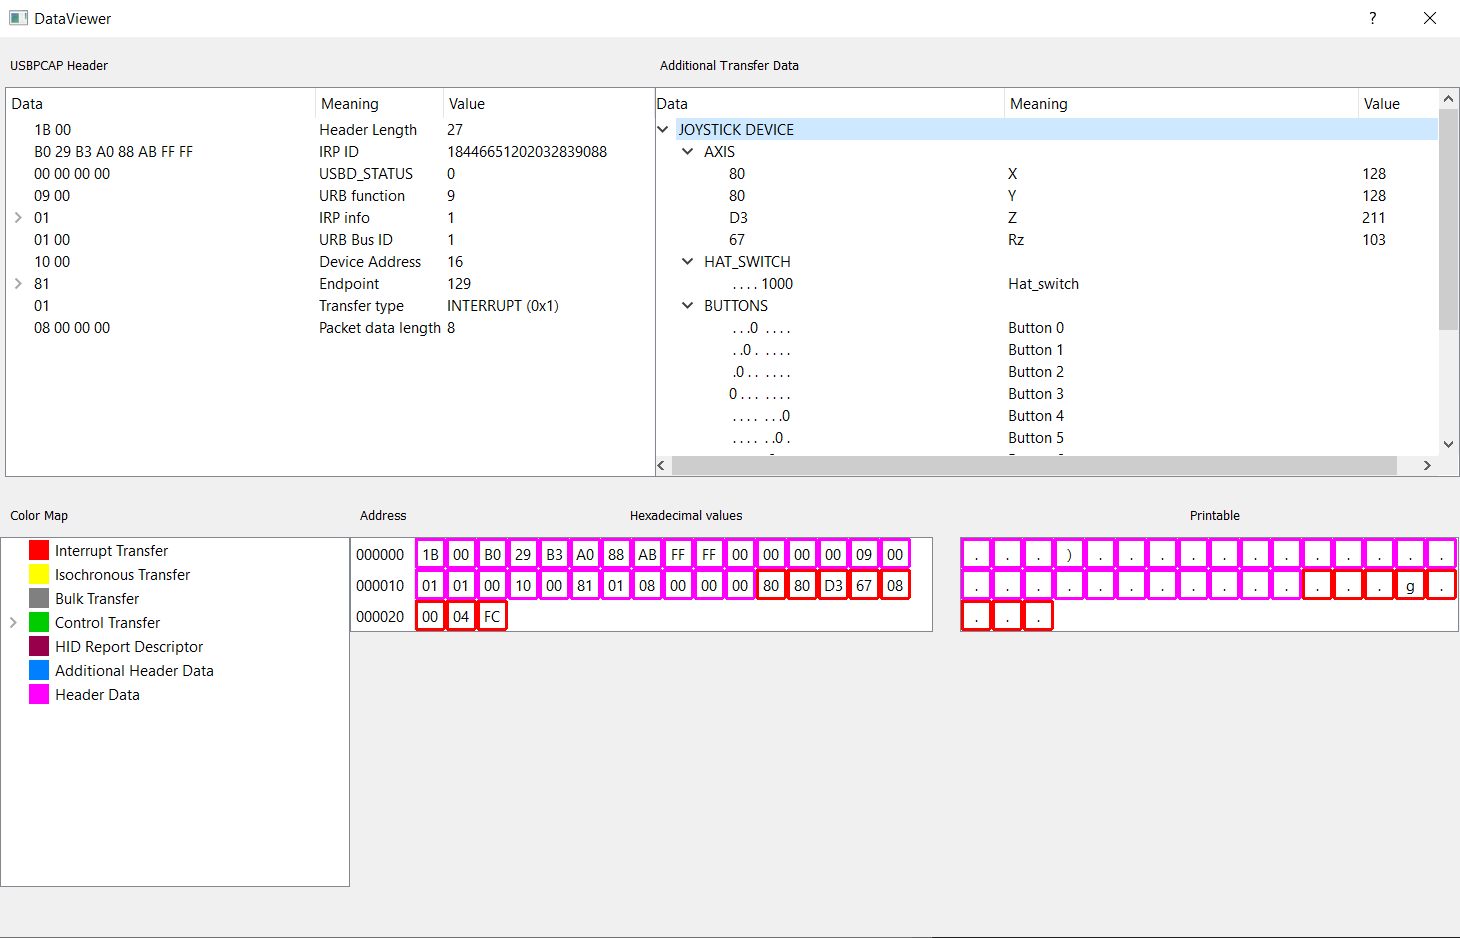
\includegraphics[width=\textwidth]{img/kap06_uk_joystick}
	\caption{Ukážka inputu joysticku.}
	\label{obr:kap6:uk_input_joystick}
\end{figure}